\documentclass[12pt]{article}

%Packages add more power to LaTeX documents
\usepackage{fullpage} %Otherwise there will be a lot of wasted space at the margins
\usepackage{enumerate} %For the multi-part problem in example #4
\usepackage{amsthm} %For proof environment
\usepackage{amsmath} %For math symbols (like the black square)
\usepackage{graphicx,float,wrapfig} %Including graphics like PDFs and some image formats.
\newcommand\tab[1][1cm]{\hspace*{#1}}

\author{John E. Buckley III}
\title{CSCI 430: Homework 2}


\begin{document}
\maketitle

\section{2.1-1}
As illustrated in class: \newline
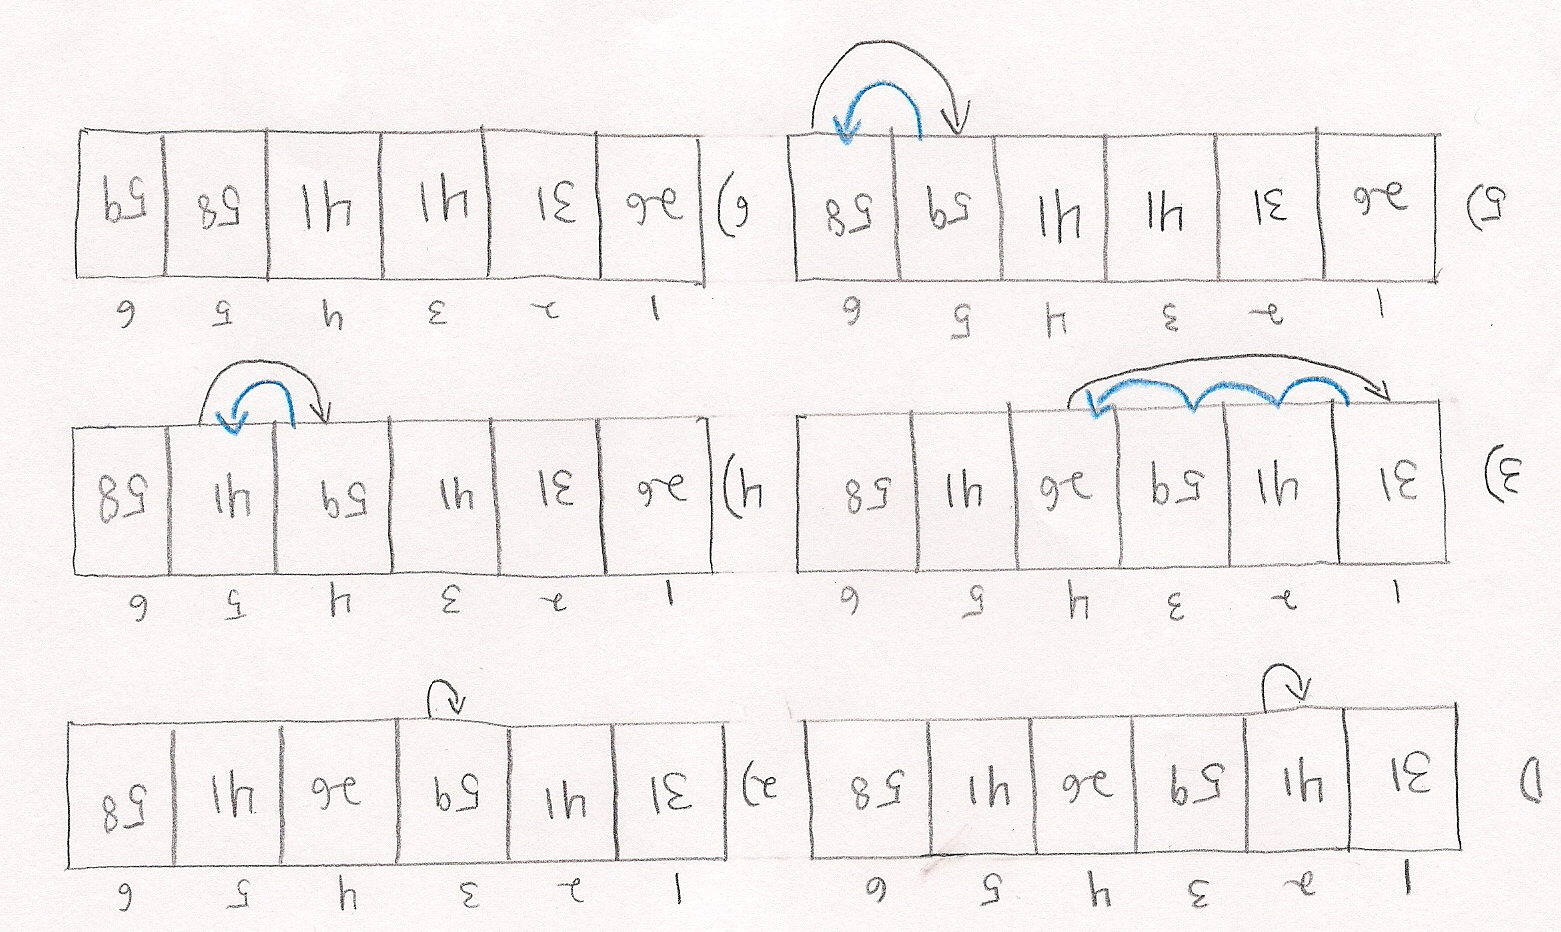
\includegraphics[scale=.75]{scan0002}

\section{2.1-2}
for $j=2$ to A.length \newline
\tab $key=A[j]$ \newline
\tab Insert $A[j]$ in to the sorted sequence $A[1...j-1]$ \newline
\tab $i=j-1$ \newline
\tab while $i>0$ and $A[i]<key$ \newline
\tab \tab $A[i+1]=A[i]$ \newline
\tab \tab $i=i-1$ \newline
\tab $A[i+1]=key$ 

\section{2.1-3}
Search$(A, v)$ \newline
\tab for $i=1$ to $A.length$ \newline
\tab \tab if $A[i]==v$ \newline
\tab \tab \tab return i \newline
\tab return NIL \newline

Loop invariant: At the start of each iteration of the for loop, the sub-array $A[1...i-1]$ consists of elements that are different than v. \newline

Proof: \newline 
Initialization: $[$We must show that the loop invariant holds before the first iteration$]$. The sub-array is initially the empty array. \newline  \newline 
Maintenance: $[$We must show that each iteration maintains the loop invariant$]$. We know that v is not in $A[1...i-1]$ so we compare it with $A[i]$ and if they are the same we will return i, otherwise we continue to the next step. \newline \newline
Termination: $[$We examine what happens when the loop terminates$]$. We terminate when $i>A.length$ and since i is increased by 1, we know that all elements in A have been accounted for and that v is not among them, thus return NIL.

\section{2.1-4}
Input: Let $A=<a_1,a_2,...,a_n>$ and $B=<b_1,b_2,...,b_n>$ be sequences of binary numbers that represent the binary integers A and B with $a_1$ and $b_1$ being the least significant bits. \newline  \newline
Output: Let $C=<c_1,c_2,...,c(n+1)>$ be a sequence of binary numbers that represent the sum of A and B with $c_1$ being the least significant bit. \newline  \newline
$SUM(A,B,C)$ \newline
\tab $carry=0$ \newline
\tab for $i=1$ to A.length \newline
\tab \tab if $(A[i]+B[i]+carry)==3$ \newline
\tab \tab \tab $carry=1$ \newline
\tab \tab \tab $C[i]=1$ \newline
\tab \tab elseif $(A[i]+B[i]+carry)==2$ \newline
\tab \tab \tab $carry=1$ \newline
\tab \tab \tab $C[i]=0$ \newline
\tab \tab elseif $(A[i]+B[i]+carry)==1$ \newline
\tab \tab \tab $carry=0$ \newline
\tab \tab \tab $C[i]=1$ \newline
\tab \tab else \newline
\tab \tab \tab $carry=0$ \newline
\tab \tab \tab $C[i]=0$ \newline
$C[i]=carry$


\end{document}